\documentclass{standalone}
\usepackage{tikz}
\usetikzlibrary{patterns, positioning}


\begin{document}
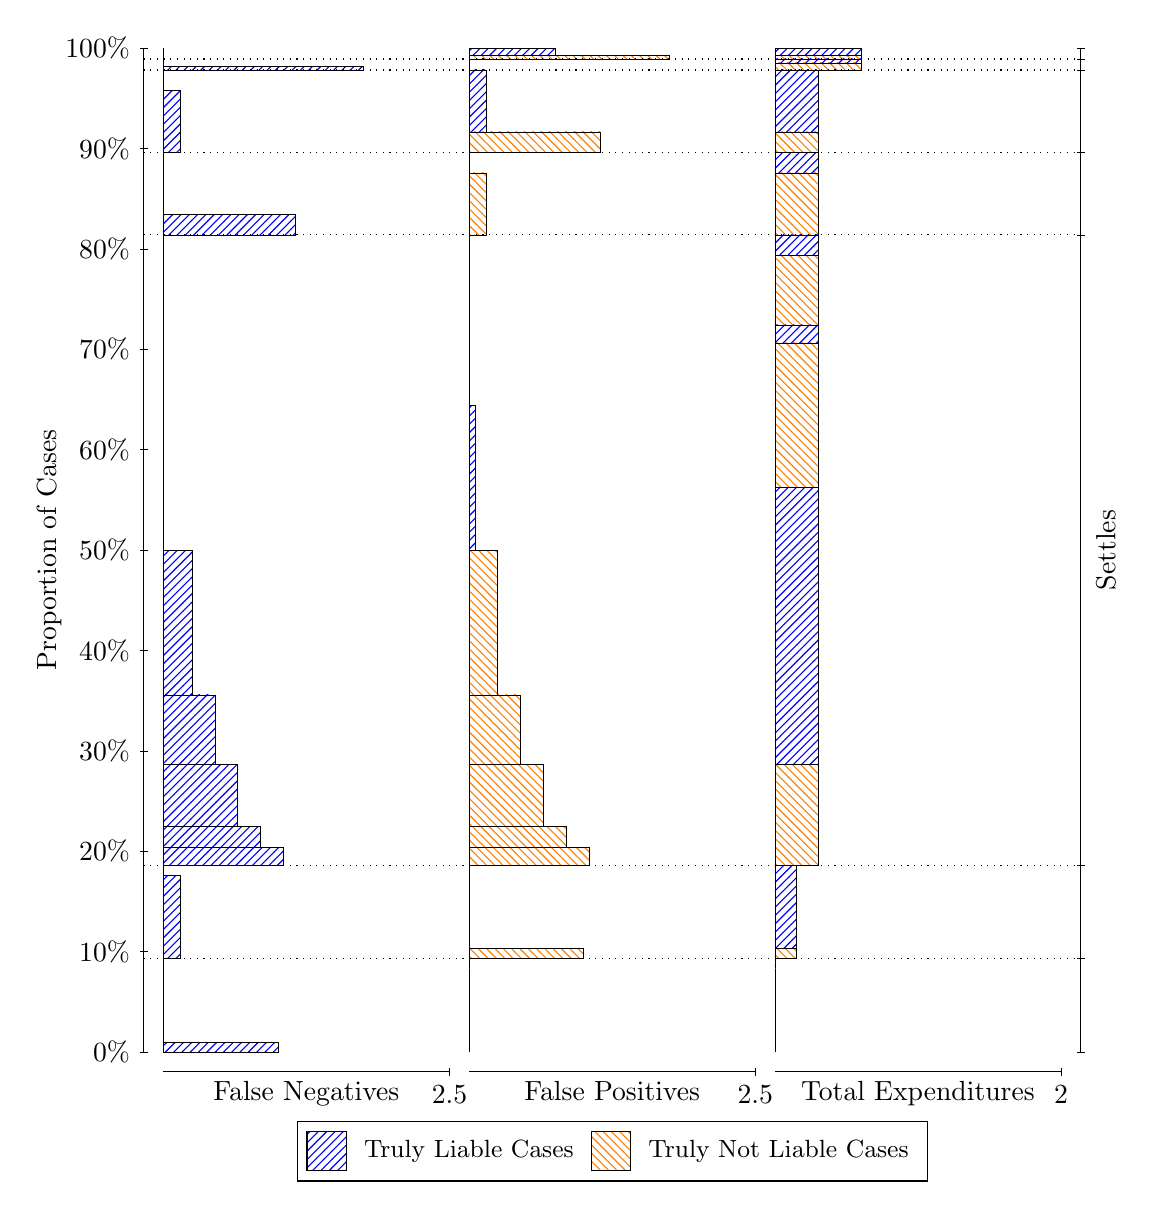
\begin{tikzpicture}
\draw[black, very thin] (1.5,1.75) -- (1.5,14.5);
\node[rotate=90, text=black, anchor=center] at (0.3, 8.125) {Proportion of Cases};
\draw[black, very thin] (1.45,1.75) -- (1.55,1.75);
\node[text=black, anchor=east] at (1.45, 1.75) {0\%};
\draw[black, very thin] (1.45,3.025) -- (1.55,3.025);
\node[text=black, anchor=east] at (1.45, 3.025) {10\%};
\draw[black, very thin] (1.45,4.3) -- (1.55,4.3);
\node[text=black, anchor=east] at (1.45, 4.3) {20\%};
\draw[black, very thin] (1.45,5.575) -- (1.55,5.575);
\node[text=black, anchor=east] at (1.45, 5.575) {30\%};
\draw[black, very thin] (1.45,6.85) -- (1.55,6.85);
\node[text=black, anchor=east] at (1.45, 6.85) {40\%};
\draw[black, very thin] (1.45,8.125) -- (1.55,8.125);
\node[text=black, anchor=east] at (1.45, 8.125) {50\%};
\draw[black, very thin] (1.45,9.4) -- (1.55,9.4);
\node[text=black, anchor=east] at (1.45, 9.4) {60\%};
\draw[black, very thin] (1.45,10.675) -- (1.55,10.675);
\node[text=black, anchor=east] at (1.45, 10.675) {70\%};
\draw[black, very thin] (1.45,11.95) -- (1.55,11.95);
\node[text=black, anchor=east] at (1.45, 11.95) {80\%};
\draw[black, very thin] (1.45,13.225) -- (1.55,13.225);
\node[text=black, anchor=east] at (1.45, 13.225) {90\%};
\draw[black, very thin] (1.45,14.5) -- (1.55,14.5);
\node[text=black, anchor=east] at (1.45, 14.5) {100\%};

\draw[black, very thin] (13.4,1.75) -- (13.4,14.5);
\draw[black, very thin] (13.35,1.75) -- (13.45,1.75);
\node[anchor=west] at (13.35, 1.75) {};
\draw[black, very thin] (13.35,2.9362) -- (13.45,2.9362);
\node[anchor=west] at (13.35, 2.9362) {};
\draw[black, very thin] (13.35,4.1223) -- (13.45,4.1223);
\node[anchor=west] at (13.35, 4.1223) {};
\draw[black, very thin] (13.35,12.127) -- (13.45,12.127);
\node[anchor=west] at (13.35, 12.127) {};
\draw[black, very thin] (13.35,13.174) -- (13.45,13.174);
\node[anchor=west] at (13.35, 13.174) {};
\draw[black, very thin] (13.35,14.221) -- (13.45,14.221);
\node[anchor=west] at (13.35, 14.221) {};
\draw[black, very thin] (13.35,14.361) -- (13.45,14.361);
\node[anchor=west] at (13.35, 14.361) {};
\draw[black, very thin] (13.35,14.5) -- (13.45,14.5);
\node[anchor=west] at (13.35, 14.5) {};

\draw[black, very thin, pattern color=blue, pattern=north east lines] (1.75,1.75) rectangle (3.2033,1.8748);
\draw[black, very thin, pattern color=orange, pattern=north west lines] (1.75,1.8748) rectangle (1.75,2.9362);
\draw[black, very thin, pattern color=blue, pattern=north east lines] (1.75,2.9362) rectangle (1.968,3.9975);
\draw[black, very thin, pattern color=orange, pattern=north west lines] (1.75,3.9975) rectangle (1.75,4.1223);
\draw[black, very thin, pattern color=blue, pattern=north east lines] (1.75,4.1223) rectangle (3.276,4.352);
\draw[black, very thin, pattern color=blue, pattern=north east lines] (1.75,4.352) rectangle (2.9853,4.6156);
\draw[black, very thin, pattern color=blue, pattern=north east lines] (1.75,4.6156) rectangle (2.6947,5.4062);
\draw[black, very thin, pattern color=blue, pattern=north east lines] (1.75,5.4062) rectangle (2.404,6.2861);
\draw[black, very thin, pattern color=blue, pattern=north east lines] (1.75,6.2861) rectangle (2.1133,8.1248);
\draw[black, very thin, pattern color=orange, pattern=north west lines] (1.75,8.1248) rectangle (1.75,12.127);
\draw[black, very thin, pattern color=blue, pattern=north east lines] (1.75,12.127) rectangle (3.4213,12.388);
\draw[black, very thin, pattern color=orange, pattern=north west lines] (1.75,12.388) rectangle (1.75,13.174);
\draw[black, very thin, pattern color=blue, pattern=north east lines] (1.75,13.174) rectangle (1.968,13.96);
\draw[black, very thin, pattern color=orange, pattern=north west lines] (1.75,13.96) rectangle (1.75,14.221);
\draw[black, very thin, pattern color=blue, pattern=north east lines] (1.75,14.221) rectangle (4.2933,14.27);
\draw[black, very thin, pattern color=orange, pattern=north west lines] (1.75,14.27) rectangle (1.75,14.361);
\draw[black, very thin, pattern color=orange, pattern=north west lines] (1.75,14.361) rectangle (1.75,14.409);
\draw[black, very thin, pattern color=blue, pattern=north east lines] (1.75,14.409) rectangle (1.75,14.5);
\draw[black, very thin, pattern color=orange, pattern=north west lines] (5.6333,1.75) rectangle (5.6333,2.8114);
\draw[black, very thin, pattern color=blue, pattern=north east lines] (5.6333,2.8114) rectangle (5.6333,2.9362);
\draw[black, very thin, pattern color=orange, pattern=north west lines] (5.6333,2.9362) rectangle (7.0867,3.061);
\draw[black, very thin, pattern color=blue, pattern=north east lines] (5.6333,3.061) rectangle (5.6333,4.1223);
\draw[black, very thin, pattern color=orange, pattern=north west lines] (5.6333,4.1223) rectangle (7.1593,4.352);
\draw[black, very thin, pattern color=orange, pattern=north west lines] (5.6333,4.352) rectangle (6.8687,4.6158);
\draw[black, very thin, pattern color=orange, pattern=north west lines] (5.6333,4.6158) rectangle (6.578,5.4065);
\draw[black, very thin, pattern color=orange, pattern=north west lines] (5.6333,5.4065) rectangle (6.2873,6.2862);
\draw[black, very thin, pattern color=orange, pattern=north west lines] (5.6333,6.2862) rectangle (5.9967,8.1247);
\draw[black, very thin, pattern color=blue, pattern=north east lines] (5.6333,8.1247) rectangle (5.706,9.9635);
\draw[black, very thin, pattern color=blue, pattern=north east lines] (5.6333,9.9635) rectangle (5.6333,12.127);
\draw[black, very thin, pattern color=orange, pattern=north west lines] (5.6333,12.127) rectangle (5.8513,12.913);
\draw[black, very thin, pattern color=blue, pattern=north east lines] (5.6333,12.913) rectangle (5.6333,13.174);
\draw[black, very thin, pattern color=orange, pattern=north west lines] (5.6333,13.174) rectangle (7.3047,13.435);
\draw[black, very thin, pattern color=blue, pattern=north east lines] (5.6333,13.435) rectangle (5.8513,14.221);
\draw[black, very thin, pattern color=orange, pattern=north west lines] (5.6333,14.221) rectangle (5.6333,14.312);
\draw[black, very thin, pattern color=blue, pattern=north east lines] (5.6333,14.312) rectangle (5.6333,14.361);
\draw[black, very thin, pattern color=orange, pattern=north west lines] (5.6333,14.361) rectangle (8.1767,14.409);
\draw[black, very thin, pattern color=blue, pattern=north east lines] (5.6333,14.409) rectangle (6.7233,14.5);
\draw[black, very thin, pattern color=orange, pattern=north west lines] (9.5167,1.75) rectangle (9.5167,2.8114);
\draw[black, very thin, pattern color=blue, pattern=north east lines] (9.5167,2.8114) rectangle (9.5167,2.9362);
\draw[black, very thin, pattern color=orange, pattern=north west lines] (9.5167,2.9362) rectangle (9.7892,3.061);
\draw[black, very thin, pattern color=blue, pattern=north east lines] (9.5167,3.061) rectangle (9.7892,4.1223);
\draw[black, very thin, pattern color=orange, pattern=north west lines] (9.5167,4.1223) rectangle (10.062,5.4065);
\draw[black, very thin, pattern color=blue, pattern=north east lines] (9.5167,5.4065) rectangle (10.062,8.9157);
\draw[black, very thin, pattern color=orange, pattern=north west lines] (9.5167,8.9157) rectangle (10.062,10.754);
\draw[black, very thin, pattern color=blue, pattern=north east lines] (9.5167,10.754) rectangle (10.062,10.984);
\draw[black, very thin, pattern color=orange, pattern=north west lines] (9.5167,10.984) rectangle (10.062,11.864);
\draw[black, very thin, pattern color=blue, pattern=north east lines] (9.5167,11.864) rectangle (10.062,12.127);
\draw[black, very thin, pattern color=orange, pattern=north west lines] (9.5167,12.127) rectangle (10.062,12.913);
\draw[black, very thin, pattern color=blue, pattern=north east lines] (9.5167,12.913) rectangle (10.062,13.174);
\draw[black, very thin, pattern color=orange, pattern=north west lines] (9.5167,13.174) rectangle (10.062,13.435);
\draw[black, very thin, pattern color=blue, pattern=north east lines] (9.5167,13.435) rectangle (10.062,14.221);
\draw[black, very thin, pattern color=orange, pattern=north west lines] (9.5167,14.221) rectangle (10.607,14.312);
\draw[black, very thin, pattern color=blue, pattern=north east lines] (9.5167,14.312) rectangle (10.607,14.361);
\draw[black, very thin, pattern color=orange, pattern=north west lines] (9.5167,14.361) rectangle (10.607,14.409);
\draw[black, very thin, pattern color=blue, pattern=north east lines] (9.5167,14.409) rectangle (10.607,14.5);
\draw[black, dotted] (1.5,2.9362) -- (13.4,2.9362);
\draw[black, dotted] (1.5,4.1223) -- (13.4,4.1223);
\draw[black, dotted] (1.5,12.127) -- (13.4,12.127);
\draw[black, dotted] (1.5,13.174) -- (13.4,13.174);
\draw[black, dotted] (1.5,14.221) -- (13.4,14.221);
\draw[black, dotted] (1.5,14.361) -- (13.4,14.361);
\draw[black, very thin] (1.75,1.5) -- (5.3833,1.5);
\node[text=black, anchor=north] at (3.5667, 1.5) {False Negatives};
\draw[black, very thin] (5.3833,1.45) -- (5.3833,1.55);
\node[text=black, anchor=north] at (5.3833, 1.45) {2.5};

\draw[black, very thin] (5.6333,1.5) -- (9.2667,1.5);
\node[text=black, anchor=north] at (7.45, 1.5) {False Positives};
\draw[black, very thin] (9.2667,1.45) -- (9.2667,1.55);
\node[text=black, anchor=north] at (9.2667, 1.45) {2.5};

\draw[black, very thin] (9.5167,1.5) -- (13.15,1.5);
\node[text=black, anchor=north] at (11.333, 1.5) {Total Expenditures};
\draw[black, very thin] (13.15,1.45) -- (13.15,1.55);
\node[text=black, anchor=north] at (13.15, 1.45) {2};



\node[text=black, centered, rotate=90] at (13.72, 8.1248) {Settles};





\draw (7.449999999999999,1.5) node[draw=none] (baseCoordinate) {};
\begin{scope}[align=center]
        \matrix[scale=0.5, draw=black, below=0.5cm of baseCoordinate, nodes={draw}, column sep=0.1cm]{
            \node[rectangle, draw, minimum width=0.5cm, minimum height=0.5cm, pattern color=blue, pattern=north east lines] {}; &
            \node[draw=none, font=\small, text=black] (B) {Truly Liable Cases}; &
            \node[rectangle, draw, minimum width=0.5cm, minimum height=0.5cm, pattern color=orange, pattern=north west lines] {}; &
            \node[draw=none, font=\small, text=black] (B) {Truly Not Liable Cases}; \\
            };
\end{scope}

\end{tikzpicture}
\end{document}